\chapter{Stand van zaken}
\label{ch:stand-van-zaken}

% Tip: Begin elk hoofdstuk met een paragraaf inleiding die beschrijft hoe
% dit hoofdstuk past binnen het geheel van de bachelorproef. Geef in het
% bijzonder aan wat de link is met het vorige en volgende hoofdstuk.

% Pas na deze inleidende paragraaf komt de eerste sectiehoofding.
Dit hoofdstuk biedt een inzicht in de huidige stand van zaken en vormt de basis voor een weloverwogen keuze bij de ontwikkeling van de PoC. Dit deel gaat zowel in op de technische als de juridische aspecten.
\\[1em]
Concreet komen de volgende onderwerpen aan bod:
\begin{itemize}
    \item \textbf{IT-support chatbot} - Wat zijn de mogelijkheden om een IT-support chatbot te maken aan de hand van een LLM en welke factoren moeten in overweging worden genomen.
    \item \textbf{De AI Act en de belangrijkste richtlijnen} - Een overzicht van de relevante wet- en regelgeving voor LLM-toepassingen.
\end{itemize}

\section{IT-support chatbot}

Om een IT-support chatbot te ontwikkelen, moeten verschillende aspecten in overweging worden genomen. Bij het gebruik van een LLM zijn er enkele belangrijke opties: Finetuning, RAG en CAG. Deze methoden maken gebruik van een LLM en verrijken de kennis van dit model met behulp van eigen documenten. Echter, elke benaderingen heeft specifieke voor- en nadelen. Het is daarom essentieel om deze zorgvuldig af te wegen om een weloverwogen keuze te maken voor de ontwikkeling van de PoC.

\subsection{Large Language Model}
    
Een LLM is een geavanceerd neuraal netwerk dat getraind is op grote hoeveelheden data om menselijke taal te kunnen begrijpen, genereren en manipuleren. LLM's gebruiken de transformer architectuur, zoals vermeld door \textcite{vaswani2023attentionneed}, die uitblinkt in het verwerken van tekst waarbij zowel de volgorde van woorden als hun contextuele relaties behouden blijven.
\\[1em]
Deze modellen worden "large" genoemd vanwege hun schaal. Ze bevatten vaak miljarden parameters. Getraind door gigantische bronnen aan data, kunnen LLM's tekst genereren die coherente, contextuele en soms zelfs creatieve eigenschappen vertoont \autocite{Gupta2025}.
\\[1em]
Hierdoor kunnen LLM’s worden ingezet voor toepassingen zoals chatbots, automatische vertaling, samenvatten van documenten en codegeneratie. Hoewel LLM’s indrukwekkende prestaties leveren, roepen ze ook vragen op. Deze hebben betrekking op een eventuele biases, hallucinatie van onjuiste informatie of het gebruik van trainingsdata die niet volledig is gecontroleerd op kwaliteit of betrouwbaarheid \autocite{Gupta2025}.
\\[1em]
De ontwikkeling van LLM’s markeert een belangrijke stap richting algemene taalintelligentie, maar roept tegelijkertijd vragen op inzake ethiek en transparantie \autocite{Gupta2025}.

\subsection{Prompting} 

Hoe goed een LLM ook presteert, de kwaliteit van de ingevoerde input heeft een grote invloed op de werking. In de context van een LLM wordt deze input aangeduid met de term prompt. Een prompt is een tekstuele template die aan het model wordt aangeboden en die het gedrag van het model stuurt met het oog op het genereren van een gewenste output. Het doel van een prompt is om de LLM te voorzien van voldoende context en duidelijke instructies om een specifieke taak uit te voeren \autocite{Marvin2024}.
\\[1em]
Voor het opstellen van een effectieve prompt bestaan verschillende technieken. Zo kan men het model extra achtergrondinformatie of richtlijnen meegeven, zodat het in staat is taken te volbrengen waarvoor het niet expliciet werd getraind. Naast de oorspronkelijke input van de gebruiker is het dus van belang om een prompt zorgvuldig te structureren en aan te vullen met relevante informatie die bijdraagt tot het behalen van het gewenste resultaat \autocite{Marvin2024}.

\subsubsection{Zero-shot vs one/few-shot learning}

Wanneer een prompt enkel instructies en/of context bevat, wordt dit aangeduid zero-shot prompting. Een andere mogelijkheid is om in de prompt één of meerdere voorbeelden op te nemen. Wanneer er één voorbeeld wordt gegeven, wordt gesproken over one-shot learning. Bij meerdere voorbeelden wordt de term few-shot learning gebruikt. Volgens \textcite{Marvin2024} helpt dit om de prestaties bij het uitvoeren van de gevraagde taak te verbeteren.
\\[1em]
\\
\subsection{Tekortkomingen van een LLM}

\subsubsection{Bias}
Bij de ontwikkeling van een LLM wordt gebruikgemaakt van grote hoeveelheden trainingsdata. Een mogelijke tekortkoming hierbij is dat de data bepaalde biases bevat. Deze kunnen tijdens de trainingsfase door het model worden overgenomen. Wanneer een LLM bijvoorbeeld wordt getraind op data met een bepaalde politieke of socio-economische voorkeuren, kan het model diezelfde biases reproduceren wanneer een gebruiker vragen stelt \autocite{Hadi2023}.
\\[1em]
Biases ontstaan echter niet uitsluitend tijdens de trainingsfase. Ook de input van gebruikers kan vooringenomenheden bevatten. Wanneer een prompt een bepaalde vooringenomenheid bevat, is het mogelijk dat de LLM deze bias overneemt of zelfs bevestigt in het gegenereerde antwoord. Dit geldt niet noodzakelijk voor elke LLM, maar het behoort zeker tot de mogelijkheden \autocite{Hadi2023}.

\subsubsection{Hallucinaties}
Hallucinaties zijn een ander probleem dat zich kan voordoen bij een LLM. Er wordt gesproken over hallucinaties wanneer een LLM een gebrek aan kennis probeert op te vullen met patronen die het model heeft geleerd tijdens het trainingsproces. Waarom een LLM gaat hallucineren, is niet altijd even duidelijk. Mogelijk ligt de oorzaak bij de training van een LLM, waarbij het model de neiging vertoont om een interessant of vloeiender antwoord te genereren voor de eindgebruiker \autocite{Hadi2023}.
\\[1em]
Dit kan echter leiden tot misleidende en foutieve antwoorden van de LLM. Het model brengt deze incorrecte informatie vaak op een manier over die zeer plausibel lijkt. Dit is potentieel zeer problematisch wanneer een LLM bijvoorbeeld wordt gebruikt in de medische wereld, waar een onnauwkeurig of misleidend antwoord verstrekkende gevolgen kan hebben \autocite{Ji2023}.

\subsubsection{Knowledge Cutoff}
Naast hallucinaties en biases is het belangrijk om te beseffen dat de kennis van het model beperkt is tot de data waarmee het werd getraind. Deze trainingsdata eindigt op een bepaald moment, wat betekent dat het model geen informatie bevat over gebeurtenissen of ontwikkelingen na die datum. Een LLM leert bovendien niet in real-time bij. Afhankelijk van de gestelde vraag kan dit leiden tot onvolledige of verouderde antwoorden. Het is daarom van belang om hiermee rekening te houden en afhankelijk van de behoeften, na te gaan wat de exacte cutoff datum is van het gebruikte model \autocite{Hadi2023}.
 
\subsection{Technieken voor kennisverrijking in LLM’s}

Er bestaan verschillende methodes om een LLM te voorzien van domeinspecifieke kennis. In dit deel worden drie van deze technieken besproken, met name RAG, Fine-tuning en CAG. 
 
\subsubsection{Retrieval Augmented Generation}

Retrieval Augmented Generation, ofwel RAG, is een techniek die een oplossing biedt voor de tekortkomingen van klassieke LLM’s. Door externe databronnen te gebruiken, kan een traditionele LLM betere resultaten behalen. Deze methode maakt het mogelijk om domeinspecifieke data te integreren en modellen bij te werken met actuele informatie. Zo kunnen klassieke LLM’s worden verrijkt met nieuwe, up-to-date gegevens die voldoen aan specifieke behoeften van de eindgebruikers \autocite{wu2025retrievalaugmentedgenerationnaturallanguage}.
\\[1em]
Om RAG in de praktijk toe te passen, moeten een aantal stappen worden doorlopen. Deze worden in het volgende deel nader toegelicht, maar samengevat bestaat het proces uit de volgende fasen:

\begin{enumerate}
    \item {Ophalen}
    \item {Verrijking}
    \item {Generatie}
\end{enumerate} 

\paragraph{Structuur en werking RAG}

Het doel van RAG is om een LLM te verrijken met specifieke kennis, zodat de gebruiker beter ondersteund wordt bij het beantwoorden van gerichte vragen. Dit proces bestaat uit drie hoofdfasen. Eerst wordt relevante informatie opgehaald. Vervolgens wordt het antwoord verrijkt op basis van de beschikbare documentatie. Tot slot genereert de LLM een antwoord op de gestelde vraag. Figuur \ref{fig:Rag process} toont hoe dit proces in zijn werk gaat.

\begin{figure}[H]
    \centering
    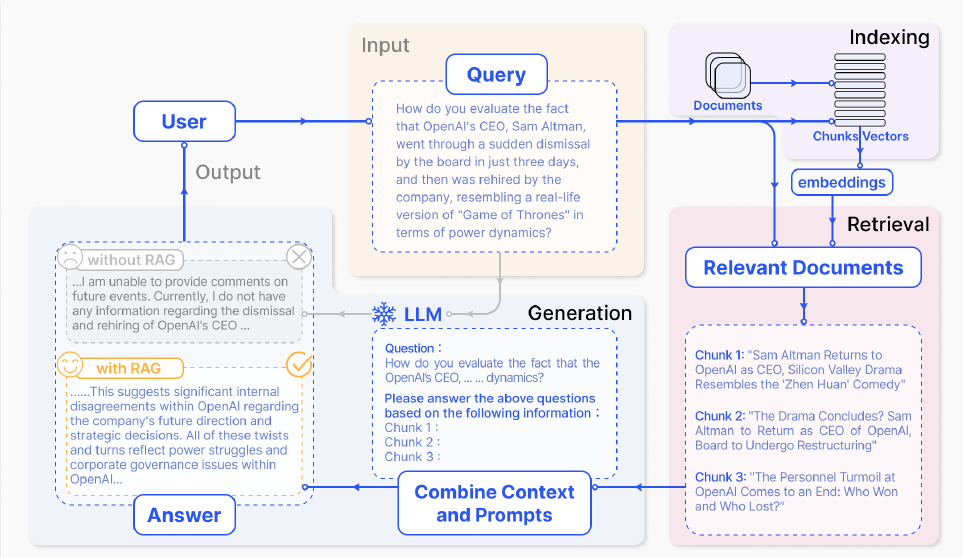
\includegraphics[width=\textwidth]{RagGao2023.png}
    \caption{Een generieke RAG architectuur \autocite{gao2024retrievalaugmentedgenerationlargelanguage}}
    \label{fig:Rag process}
\end{figure}

\subparagraph{Ophalen}
Voordat de LLM effectief bevraagd kan worden over domeinspecifieke informatie, moet eerst grondig voorbereidend werk plaatsvinden. 
\\[1em]
De documenten worden niet in hun geheel, maar in kleinere segmenten verwerkt, zogenaamde "chunks". Het opdelen in tekstsegmenten is noodzakelijk omdat volledige documenten doorgaans te omvangrijk zijn om efficiënt te verwerken binnen de contextlimieten van een LLM. Bovendien maakt deze fragmentatie het mogelijk om op een meer gerichte manier informatie op te halen uit de vectordatabase \autocite{wu2025retrievalaugmentedgenerationnaturallanguage}.
\\[1em]
Voor het opdelen van documenten bestaan verschillende benaderingen. Een veelgebruikte techniek is het verdelen van tekst op basis van een vooraf bepaald aantal tokens of karakters, zodat elke chunk ongeveer dezelfde lengte heeft \autocite{wang2024searchingbestpracticesretrievalaugmented}.
\\[1em]
Een alternatieve strategie, die vooral geschikt is voor tekstuele documenten, is het opdelen op basis van zinnen of alinea's. Deze aanpak draagt doorgaans bij aan het behoud van de semantische samenhang binnen een chunk. Dit komt de kwaliteit van de informatieophaling ten goede \autocite{wang2024searchingbestpracticesretrievalaugmented}.
\\[1em]
Na het opdelen worden deze tekstsegmenten omgezet in zogeheten embeddings. Dit zijn vectorrepresentaties die de semantische inhoud van de chunks op een numerieke manier vastleggen. Deze embeddings worden vervolgens opgeslagen in een vectordatabase. Dit is een specifiek type databank dat geoptimaliseerd is voor het bewaren en efficiënt ophalen van vectorrepresentaties. Dit gehele proces vormt de basis waarop de LLM tijdens het beantwoorden van vragen relevante context uit de vectordatabase kan ophalen \autocite{wu2025retrievalaugmentedgenerationnaturallanguage}. Figuur \ref{fig:RAG opmaken vectordatabase} illustreert dit proces.

 \begin{figure}[H]
    \centering
    \includegraphics[width=\textwidth]{retrieverWu2024.png}
    \caption{Documentverwerking en opslag in een vectordatabase via embeddings \autocite{wu2025retrievalaugmentedgenerationnaturallanguage}}
    \label{fig:RAG opmaken vectordatabase}
\end{figure}

Zodra de documenten via embeddings zijn toegevoegd aan de vectordatabase kan een gebruiker de LLM bevragen over deze documenten. Een vraag of query wordt net als de documenten vertaald naar embeddings. Op basis van deze representaties worden de top-k dichtstbijzijnde buren opgehaald, oftewel de meest relevante delen van de opgeslagen documenten \autocite{wu2025retrievalaugmentedgenerationnaturallanguage}. Figuur \ref{fig:RAG bevragen vectordatabase} illustreert hoe dit proces precies verloopt.
        
\begin{figure}[H]
    \centering
    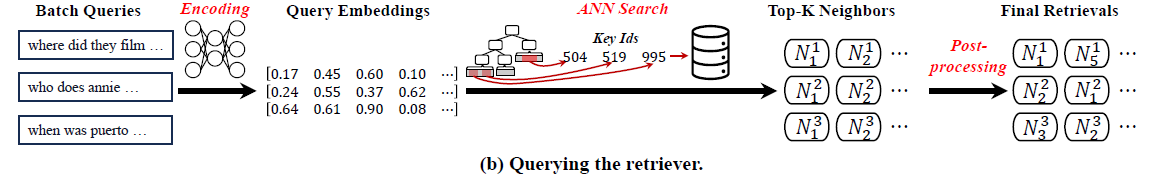
\includegraphics[width=\textwidth]{QueryRetrieverWu2024.png}
    \caption{Vraagafhandeling en ophalen van relevante chunks \autocite{wu2025retrievalaugmentedgenerationnaturallanguage}}
    \label{fig:RAG bevragen vectordatabase}
\end{figure}

\subparagraph{Verrijking en Generatie}

Zodra de meest relevante informatie is opgehaald, wordt deze gebruikt in het antwoordproces. De opgehaalde documenten worden, samen met de vraag van de gebruiker, toegevoegd aan de context van het model. Hierdoor beschikt de LLM over aanvullende informatie en kan de vraag nauwkeuriger worden beantwoord. Het resultaat is een antwoord dat gebaseerd is op de geïnjecteerde kennis uit de vectordatabase \autocite{zhao2024retrievalaugmentedgenerationaigeneratedcontent}.


\subsubsection{Fine-tuning}

Fine-tuning probeert hetzelfde probleem op te lossen als RAG, namelijk dat een LLM geen of onvoldoende domeinkennis heeft om bepaalde vragen te antwoorden. De manier waarop dit wordt opgelost is echter anders. Bij fine-tuning wordt een bestaande LLM verder getraind met een eigen dataset. Met andere woorden, het doel is om de parameters van het model aan te passen, zodat het model accurater kan antwoorden op domeinspecifieke vragen \autocite{Raj2024}.
\\[1em]
Wanneer een model is bijgesteld, kan het domeinspecifieke vragen beantwoorden zonder dat het daarbij een vectordatabase nodig heeft. De domeinspecifieke kennis wordt als het ware ingebakken in het model, waardoor het niet meer afhankelijk is van externe kennisbronnen \autocite{Raj2024}.
\\[1em]
Hoewel fine-tuning zeker een techniek is die heeft aangetoond te werken, moet er wel rekening worden gehouden met de hoge initiële kosten, vooral in vergelijking met een oplossing zoals RAG. Daarnaast speelt ook het feit dat er een minimale hoeveelheid data nodig is om een model te trainen. Fine-tuning is mogelijk met kleinere datasets, maar het is efficiënter bij grotere datasets \autocite{Balaguer2024}.

\subsubsection{Cache-Augmented Generation}

Met de opkomst van nieuwe LLM's die een grotere context bevatten is het niet altijd nodig om te werken met een RAG-architectuur. Wanneer het aantal documenten en de lengte ervan niet dermate groot zijn kan je ook meteen alle documenten injecteren in de context van een LLM. Dit zorgt voor een heel simpele en efficiënte benadering om een LLM bedrijf- of contextspecifieke kennis te geven \autocite{Chan2025}.
\\[1em]
Het voordeel van deze aanpak is dat een deel van het RAG-proces wordt geëlimineerd, met name de documentatie moet niet meer worden opgeslagen in een vectordatabase \autocite{Chan2025}. 
\\[1em]
Er is ook niet langer nood aan het ophalen van de geselecteerde gegevens wat mogelijks fouten binnen dit proces ook elimineert. Dit is dus zeker een valabele optie wanneer het gaat over een beperkte verzameling van documentatie \autocite{Chan2025}. 
\\[1em]
Een potentieel gevaar bij het gebruik van CAG is echter zogenaamde context rot. Volgens \textcite{hong2025context} neemt de performantie van een LLM af wanneer meer informatie aan de context wordt toegevoegd. Hoewel de nieuwste modellen een context window hebben van soms wel een miljoen tokens, is het daarom niet aan te raden dit volledig te benutten. Gelet op de negatieve impact die dit kan hebben op de prestaties van het model zelfs voor simpele vragen.

\subsection{LLM benchmarks}
Om te bepalen welke modellen het meest geschikt zijn voor de ontwikkeling van IT-support chatbot, is een objectieve meetmethode noodzakelijk. Gelukkig bestaan er verschillende platformen die LLM's vergelijken en rangschikken op basis van prestaties in verschillende categorieën. In deze sectie worden enkele van deze platformen besproken.
   
\subsubsection{LiveBench} 
Een platform dat LLM's evalueert, is LiveBench. Deze site stelt een rangschikking op voor verschillende modellen en biedt een actuele scorebord die elke zes maanden wordt bijgewerkt. Voor deze bachelorproef zal gebruik worden gemaakt van de ranking afkomstig uit de paper gepubliceerd in april 2025 \autocite{livebench}.
\\[1em]
LiveBench beoordeelt LLM's op basis van zes categorieën. Binnen elke categorie worden meerdere taken uitgevoerd om een nauwkeurige beoordeling te verkrijgen. De zes categorieën zijn:
\begin{itemize}
    \item Wiskundige vaardigheden (Math)
    \item Programmeervaardigheden (Coding)
    \item Redeneren en probleemoplossing (Reasoning)
    \item Data-analyse (Data Analysis)
    \item Volgen van instructies (Instruction Following)
    \item Begrip van natuurlijke taal (Language Comprehension)
\end{itemize}

Elke categorie wordt geëvalueerd op basis van specifieke taken. Dit resulteert uiteindelijk in een algemene rangschikking, waarin zowel de beste modellen per categorie als het beste presterende model in het algemeen worden geïdentificeerd. Figuur \ref{fig:livebench} toont deze evaluatie op een overzichtelijke manier \autocite{livebench}.

\begin{figure}[H]
    \centering
    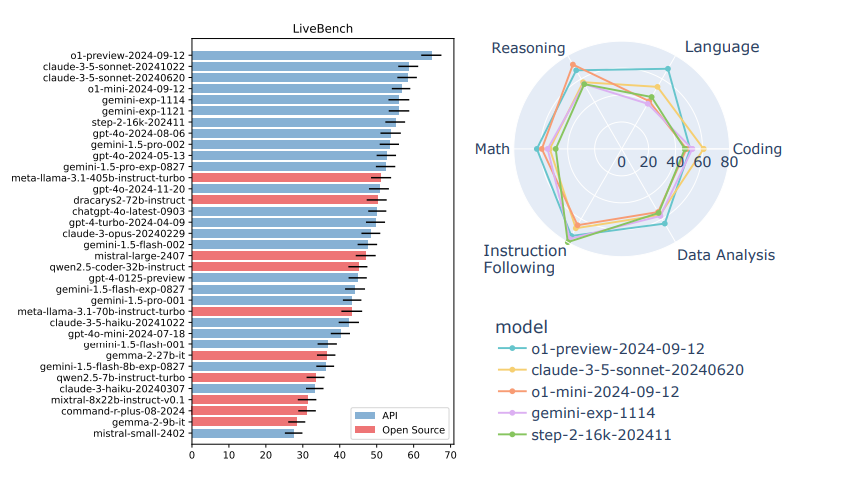
\includegraphics[width=\textwidth]{LiveBenchRanking.png}
    \caption{LiveBench ranking van verschillende LLM's.}
    \label{fig:livebench}
\end{figure}

Uit de ranking van LiveBench kan geconcludeerd worden dat 3 verschillende organisaties elk een model aanbieden die vanuit globaal oogpunt tot de top 3 behoort. Deze top 3 zijn: 
\begin{enumerate}
    \item o1-preview-2024-09-12 van OpenAI
    \item claude-3-5-sonnet-20241022 van Anthropic
    \item claude-3-5-sonnet-20240620 van Anthropic
\end{enumerate}

\subsubsection{Chatbot Arena} 

Een andere benchmark tool is Chatbot Arena, net zoals LiveBench is Chatbot Arena een site die een actuele weergave biedt van de beste LLM's op basis van vooraf gedefinieerde categorieën. 
Volgens de ranking van \textcite{chiang2024chatbotarenaopenplatform} zijn dit de top 3 LLM's:

\begin{enumerate}
    \item GPT-4-Turbo van OpenAI
    \item GPT-4-0613 van OpenAI
    \item Mistral-Medium Mistral AI
\end{enumerate}

Hoewel het doel van beide benchmarks hetzelfde is, hanteert elke benchmark een andere werkwijze. Bij Chatbot Arena krijgen gebruikers twee anonieme modellen tegenover elkaar geplaatst. De gebruiker kan vervolgens een eigen vraag stellen en bepaalt zelf welk van de twee modellen het beste resultaat levert.
\\[1em]
Het voordeel van deze methode is dat de LLM's realistische cases moeten behandelen, gebaseerd op vragen die daadwerkelijk door gebruikers worden gesteld. Op basis van de resultaten kunnen gebruikers hun voorkeur aangeven. Een nadeel is dat de deelnemers van deze testen vaak niet representatief zijn voor alle LLM-gebruikers. Dit zijn meestal mensen met een speciale interesse in LLM's of onderzoekers in het vakgebied. Desondanks maakt deze methode het mogelijk om verschillende modellen met elkaar te vergelijken. In januari 2024 werden ruim 240.000 stemmen uitgebracht door ongeveer 90.000 gebruikers \autocite{chiang2024chatbotarenaopenplatform}. 

\subsubsection{Conclusie}

Op basis van de twee besproken benchmarks kan niet eenduidig worden bepaald welke modellen het beste presteren. De omgeving is immers zeer dynamisch en snel veranderend, waardoor modellen die vandaag de beste resultaten leveren over een maand mogelijk al door nieuwere modellen worden overtroffen. Desalniettemin bieden deze benchmarks waardevolle informatie en inzichten over de sterke punten van bepaalde modellen ten opzichte van andere.

\subsection{Evaluatiemethoden voor LLM-output}
Het gebruik van een performante LLM volstaat op zich niet. Minstens even belangrijk is het evalueren van de kwaliteit en accuraatheid van de gegenereerde antwoorden. Hiervoor bestaan er verschillende evaluatiemethoden, waaronder de Bilingual Evaluation Understudy (BLEU), de Recall-Oriented Understudy for Gisting Evaluation (ROUGE), en BERTScore \autocite{microsoft2024evaluation}.
\\[1em]
Deze methoden kennen elk hun eigen berekeningswijze, maar delen een belangrijk gemeenschappelijk kenmerk. Ze zijn allen afhankelijk van de aanwezigheid van een referentie-antwoord. Dit referentie-antwoord wordt gebruikt als maatstaf om de gegenereerde output van de LLM mee te vergelijken en zo een score toe te kennen die de kwaliteit van de output reflecteert\autocite{microsoft2024evaluation}.

\subsubsection{BLEU Score}

De BLEU score is een evaluatie metriek die oorspronkelijk werd ontwikkeld om de kwaliteit van door machines gegenereerde vertalingen te beoordelen. Hierbij wordt de output van het model vergeleken met een of meerdere menselijke referentievertalingen. Aan de hand van overlappingen of zogenaamde n-gram overeenkomsten, reeksen van één of meerdere opeenvolgende woorden, wordt een score toegekend. De score ligt tussen 0 en 1, waarbij een hogere score duidt op een grotere overeenkomst met de referentietekst \autocite{papineni-etal-2002-bleu}.
\\[1em]
Een score van 1 betekent een perfecte overeenkomst, maar zelfs menselijke vertalingen behalen zelden deze score. Aangezien er vaak meerdere correcte vertaalmogelijkheden bestaan die kunnen afwijken. Hoewel BLEU een snelle en reproduceerbare maat biedt voor evaluatie, heeft het beperkingen doordat het geen rekening houdt met betekenis en contextuele variatie \autocite{papineni-etal-2002-bleu}.

\subsubsection{ROUGE Score}

Net zoals de BLEU-score evalueert de ROUGE-score de mate van overlap tussen een door machine gegenereerde tekst en een menselijke referentie. Waar BLEU echter voornamelijk gericht is op de precisie van exacte n-gram overeenkomsten, focust ROUGE sterker op de inhoudelijke dekking van de referentie. Hierdoor biedt de ROUGE-score een diepgaander inzicht in de kwaliteit van het gegenereerde antwoord \autocite{ganesan2018rouge20updatedimproved}.

\subsubsection{BERTScore}

BERTScore is een automatische evaluatiemethode voor tekstgeneratie. In tegenstelling tot traditionele methoden zoals BLEU, maakt BERTScore gebruik van contextuele embeddings van het taalmodel BERT. Daarmee worden semantische gelijkenissen tussen tokens vergeleken. Hierdoor is deze metriek beter in staat om betekenisovereenkomsten te herkennen, zelfs wanneer een andere woordkeuze of zinsstructuur wordt gebruikt. Met andere woorden: BERTScore benadert menselijke beoordelingen beter dan bestaande meetcriteria zoals BLEU \autocite{Zhang2019}.

\subsection{Evaluatieframework voor retrieval-gebaseerde LLM-systemen}

Specifiek voor LLM-systemen die gebruikmaken van externe bronnen, zoals bij RAG, bestaan er frameworks om de kwaliteit van het gegenereerde antwoord te beoordelen. Een voorbeeld hiervan is Retrieval Augmented Generation Assesment of \textit{Ragas}. Ragas biedt verschillende mogelijkheden om zaken te testen die relevant zijn binnen een RAG-proces \autocite{Es2023}. Deze zaken zijn:
\begin{enumerate}
    \item Faithfullness
    \item Answer Relevance
    \item Context Relevance
\end{enumerate}

Faithfulness (feitelijke correctheid) richt zich op het feit dat het door de LLM gegenereerde antwoord voortvloeit uit de opgehaalde context. Met andere woorden, de LLM moet zijn antwoord baseren op de relevante documenten die tijdens het ophaalproces zijn opgehaald. Zo kan worden nagegaan of de LLM geen hallucinaties produceert, iets wat in een RAG-proces ten allen tijde vermeden moet worden \autocite{Es2023}.
\\[1em]
Answer Relevance (Antwoord relevantie) is een tweede evaluatiemetriek, hier wordt nagegaan of het gegenereerde antwoord relevant is voor de vraag die werd gesteld. Hiernaast zal ook worden nagegaan of het antwoord geen overbodige informatie bevat. De modellen krijgen met andere woorden minder punten indien te veel onnodige informatie wordt toegevoegd aan het antwoord \autocite{Es2023}.
\\[1em]
Het derde en laatste meetinstrument is Context Relevance (context relevantie). Hierbij wordt nagegaan hoe relevant de context is tegenover de gestelde vraag. Net zoals bij antwoord relevantie zal de score minder hoog zijn wanneer er een onnodige context aanwezig is die niet relevant zijn voor de vraag \autocite{Es2023}. 
\\[1em]
Elke metriek krijgt een score tussen 0 en 1, waarbij 1 een perfecte prestatie binnen de betreffende categorie aangeeft en 0 het tegenovergestelde \autocite{Es2023}.

\section{De AI Act en de belangrijkste richtlijnen}
De AI Act is een regelgevend kader van de Europese Commissie dat juridische richtlijnen biedt voor het gebruik van artificiële intelligentie. Het doel van deze wetgeving is het beperken van bepaalde risico’s die AI-systemen met zich meebrengen en het voorkomen van ongewenste effecten \autocite{EUAIAct2024}.
\\[1em]
Binnen de AI Act worden AI-toepassingen ingedeeld in vier risiconiveaus. Afhankelijk van de toepassing valt het systeem in één van deze categorieën en moet het voldoen aan de bijbehorende regels. De eerste categorie omvat praktijken die als onaanvaardbaar worden beschouwd. Met andere woorden, dit zijn toepassingen die volgens deze wetgeving binnen de EU verboden zijn \autocite{EUAIAct2024}.
\\[1em]
Een tweede categorie betreft hoog risico AI-systemen. Deze systemen zijn toegestaan, maar mogen alleen worden gebruikt onder strikte voorwaarden. Het hoge risico kan voortkomen uit het doel van het systeem, de context waarin het wordt ingezet, of de mogelijke impact op fundamentele rechten. Bijvoorbeeld een AI-systeem dat wordt gebruikt om rechtszaken voor te bereiden wordt als hoog risicovol beschouwd. Dit komt omdat het de fundamentele rechten van burgers kan beïnvloeden \autocite{EUAIAct2024}.
\\[1em]
De voorlaatste categorie betreft AI-systemen met beperkte risico’s. Dit kan bijvoorbeeld gaan over chatbots. Binnen deze categorie legt de AI Act vooral de nadruk op transparantie. Wanneer een AI-systeem tot deze categorie behoort, moet de gebruiker hiervan op de hoogte worden gesteld. Op die manier weet de gebruiker altijd of hij of zij met een AI-systeem communiceert \autocite{EUAIAct2024}.
\\[1em]
De laatste categorie betreft AI-systemen met geen of minimale risico’s. Voor deze systemen worden geen specifieke regels opgelegd, omdat ze weinig tot geen risico vormen. Dit gaat bijvoorbeeld over spamfilters \autocite{EUAIAct2024}.
\\[1em]
De AI Act bevat naast de risiconiveaus ook specifieke regels voor generatieve AI. Vanwege de aard van generatieve AI kunnen toepassingen onder meerdere van de eerder besproken categorieën vallen. Ongeacht de categorie moeten bedrijven die LLM’s produceren transparantie bieden over de gebruikte trainingsdata. Wanneer deze LLM’s worden ingezet in hoog risico systemen, gelden extra verplichtingen. Zowel de ontwikkelaars van het systeem als de makers van de LLM moeten samenwerken om deze risico’s zoveel mogelijk te beperken. Zodra het product op de markt komt, ligt ook bij de organisaties die deze tools gebruiken een verantwoordelijkheid om de risico’s te minimaliseren \autocite{EUAIAct2024}.
\\[1em]
Samengevat biedt de AI Act een kader om het gebruik van AI op een veilige en transparante manier te reguleren. Door het indelen van toepassingen in verschillende risiconiveaus en het opleggen van specifieke verplichtingen, probeert de wetgeving zowel de ontwikkeling van AI te stimuleren als de fundamentele rechten van burgers te beschermen. Dit zorgt ervoor dat organisaties bewust omgaan met de risico’s van hun AI-systemen, ongeacht of het gaat om generatieve AI of andere toepassingen \autocite{EUAIAct2024}.